\section{Implementation}

This chapter will cover the implementation process as well as a detailed description of the final implementation of the application.

\subsection{Introduction}

The main application consists of different views, extending the Android Activity class, and several helper and model classes. All examination data is stored in an SQLite database, and can be presented as individual examinations using the \emph{Examination} model class. The application uses an AIDL to communicate with a service specified in the application settings. This service is made for each hospital to account for the difference in standards and servers used.

\subsubsection*{Android Development Terminology}
This section will cover a few terms used in this document for readers unfamiliar with the Android development platform.

An \emph{Activity} is defined as a single, focused thing that the user can do. Almost all activities interact with the user in some way, and are in most cases a single view with UI elements. To start activities and services an \emph{Intent} is used. The \emph{Intent} is an abstract description of an operation to be preformed, and works as a passive data structure to transport data between different activities.

The application \emph{Context} is an interface to global information about the application environment. This is used to access the same SharedPreferences from different activities within the application. \emph{SharedPreferences} is a local storage space offered by the Android operating system where \emph{key, value pairs} of primitive data types can be permanently stored.

A Service is a component that runs without any user interaction, and is designed to do long-running operations in the background. A \emph{ServiceConnection} is used to communicate with the service. To start using a service, the \emph{bindService()} method is called. If the service is bound successfully, it will return an \emph{IBinder} object that can be used to communicate with the service.

AIDL (Android Interface Definition Language) is an interface language used to define general interface structures for service communication. It is used to communicate with services outside of the application itself. When the \emph{.aidl} file is compiled for Java, it will create a Java interface class that will act as a service.

\subsection{Implementation Details}

This section will describe how the different parts of the application were implemented and how the different modules interact with each other. A complete overview of the different packages and their relation can be found in the Appendix \ref{classdiagram}.

\subsubsection{Initial Setup}

Before the application can be used, it has to be configured to work with the correct hospital. As the application itself is dependent on several settings that the normal user not necessarily will have access to, it is required that the application is set up by technical personnel before use. These settings range from hospital server addresses, to department credentials and authentication variables.

Figure \ref{fig:config} illustrates the scenario where the technical user starts the application for the first time, sets a password for restricted access to the "Settings"-view, and configures the application with a preconfigured settings file. This file is downloaded from a hospital HTTP server.  

\begin{figure}[H]
\centering
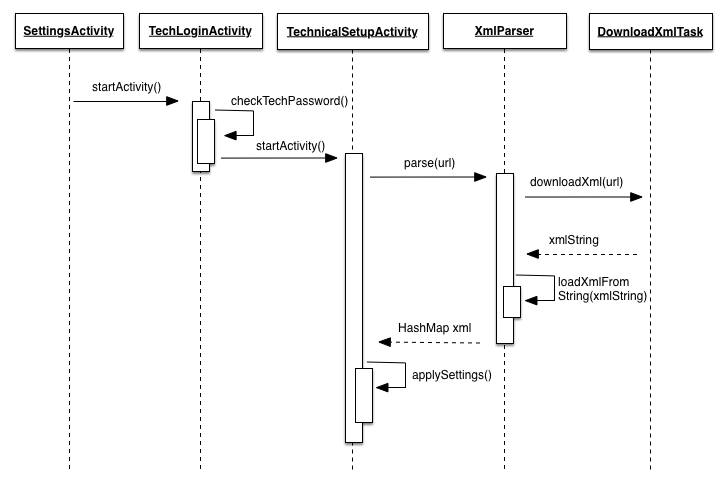
\includegraphics[scale=0.5]{img/sequence_config.png}
\caption{First time configuration}
\label{fig:config}
\end{figure}

\subsubsection{User Interface}
\label{viewholderImp} 

After the initial setup, the only way to start the application is through the Vscan application. As the Vscan application was not a part of the project, the \emph{GatewayLauncher} class was created as a template for launching the application.

The "Login"-view is the first view presented to the user no matter which launcher method is used, and the \emph{LoginActivity.java} will redirect the user to different parts of the application, depending on the information from the launcher. The most important part of the launcher is the first four static variables. These variables tells the LoginActivity which part of the application to start. The different constructors are there to ensure that the correct information is provided for the different launch modes. More information about the different launch modes will be covered in section \ref{appworkflow}.

To implement MVC we used an \emph{Examination} class as the model for each examination. The \emph{ExaminationActivity} is both view and controller for this model while \emph{HomeScreenActivity} and \emph{ReviewAndUploadActivity} only serves as views. The second model is the \emph{EMRApplication} class, which holds all application settings. \emph{CurrentSetupActivity} is used to view this model, and \emph{TechnicalSetupActivity} is used as a controller.

For showing data in a scrollable list, a \emph{ListView} is used. A ListView is, like the name suggests, a view group of elements that together constitutes a list. A ListView can contain any number of elements. In Android, an \emph{Adapter} acts as a bridge between the ListView and the data it displays. Figure 16 shows the relationship between the adapter, underlying data and an activity. When an user scrolls the ListView, the adapter's \emph{getView(...)} method is called. This method will repeatedly call \emph{findViewById(...)}, which retrieves layout widgets in the UI. The \emph{getView}-method will then return a View and tell the ListView to display it. This happens for every row visible on the screen as well as the next and previous rows to be shown \cite{adapter}. When dealing with a large amount of data, this may cause scrolling ListViews to be slow and choppy due to the \emph{findViewById(...)}-method being called repeatedly. This is where the ViewHolder pattern comes in \cite{viewholder}. The ViewHolder is told to hold the layout widgets so they don't have to be retrieved time after time with the \emph{findViewById(...)}-method. Listing \ref{lst:viewholder} shows the implementation of ViewHolder pattern in \emph{ReviewListAdapter.java}.

\newpage

\begin{lstlisting}[caption={ViewHolder implementation}, label={lst:viewholder}]
// ReviewListAdapter.java
private LayoutInflater inflater;

static class ViewHolder {
    TextView imageDateTextView ;
    TextView commentTextView;
    ImageView rowImage;
}

@Override
public View getView(int position, View convertView, ViewGroup parent) {

    ViewHolder holder;

    if (convertView == null) {
        convertView = inflater.inflate(resource, null);

        holder = new ViewHolder();
        holder.imageDateTextView = (TextView) convertView.findViewById(R.id.imageDate);

        convertView.setTag(holder);
    } else {
        holder = (ViewHolder) convertView.getTag();
    }
    return convertView;
    }
}
\end{lstlisting}

\noindent
The call to \emph{findViewById()} happens at line 21, and the ViewHolder is told to hold the \emph{TextView}. The next time \emph{getView()} is called, the method will not have to call \emph{findViewById()}. This will greatly improve performance, especially with large lists.

\begin{figure}[H]
        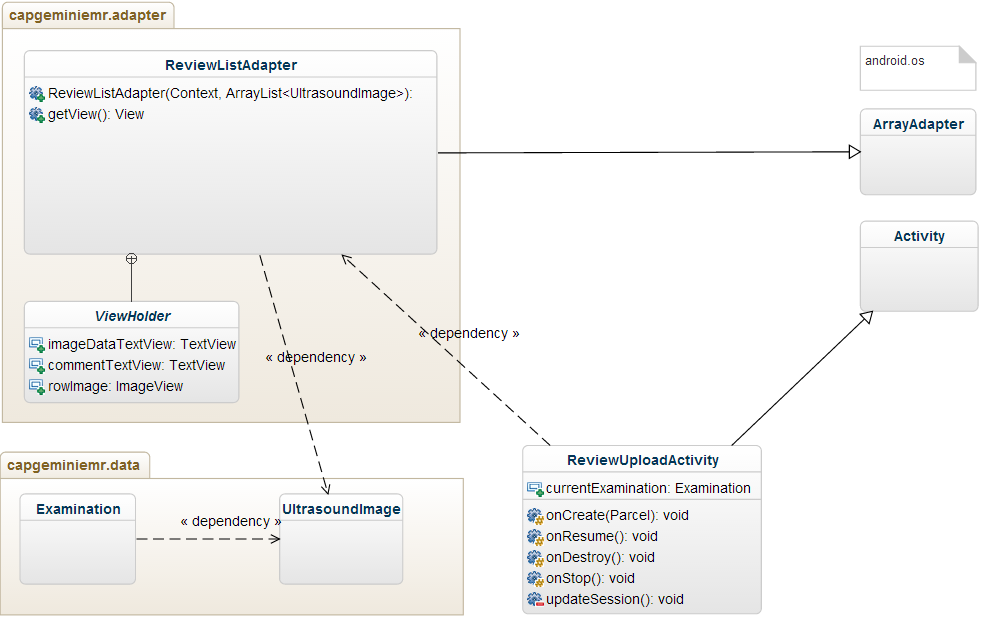
\includegraphics[scale=0.5]{img/classdiagram2.png}
        \caption{Relationship ListAdapter, data and Activity}
    \label{classdiagram_data_adapter}
\end{figure}


\paragraph{Application workflow}
\label{appworkflow}

Disregarding the technical views, the application is designed to have a very linear flow, where the user is guided step-by-step through the process of preparing and uploading the examination. As the application itself is only reachable through the Vscan application, there are three different ways for the application to behave. 

In the first scenario, the user only wishes to identify the patient prior to an examination. Given this scenario, the application launches, the user logs in and inputs or scans the patients SSN. If the SSN is recognized, the application returns the patient information back to the Vscan application, and the application finishes. 

In the second scenario, the user wishes to conduct and upload an examination. Data from the examination is used to launch the application. Dependent upon if the scenario above has taken place, the user either inputs (or scans) the patient's SSN, or the application automatically utilizes the information retrieved from the first scenario. The user then arrives at the "Examination"-view, where he is given an overview over the patient's information, and is given the option to add a comment on the examination as a whole, as well as the option to review the images. By choosing to review the images from the examination, a full screen view of the images are presented to the user, where the user can zoom in on images for further inspection, swipe between them, delete images not to be uploaded, and add comments to each image. When the user is done, the full screen view can be closed by clicking the "close"-button, which returns the user to the "Examination"-view. 

The "Examination"-view informs the user of the number of images lacking a comment. This is a part of the design feature, intended to ensure that all images uploaded by the user, is of diagnostic value, mentioned in section \ref{multimediaInHospitals}.

When done, the "Review and Upload"-button takes the user to the view with the same name. The view is designed with the same intention as above, forcing the user to scroll through each image of the examination. At the bottom of the list, the user is presented with the option to either edit the examination, taking the user back to the "Examination"- view, or to upload the examination. If the user chooses the latter option, a dialog will alert the user if any images lacks comments. 
After the potential dialog has been disregarded, the process of uploading the examination is initiated. After completion, the user is returned to the "Not yet Uploaded"- view (described in details bellow).

In the third scenario, the user wishes to view stored examinations. After login, the user is sent to the "Not yet Uploaded"-view, where all examinations are listed. The user here has the option to either delete or upload the examinations. 

Common to the scenarios above, is that if the application for any reason detects either network loss or session timeout, all sensitive data is stripped from the views. The user is still able to enter sensitive data, but is not able to see information already entered.


\subsubsection{Database}
\label{databaseImp}

The need for a local database is mainly rooted in the fact that the application should be working offline. Additionally, having progress be stored at key points in the application flow ensures that work is never lost should the application unexpectedly close or be terminated after these key points. As mentioned earlier, the database is encrypted because it contains sensitive data. This may lead to a performance problem, especially on older and slower devices.

Figure \ref{fig:database_design} shows the database design. It consists of two tables; \emph{Examination} and \emph{UltrasoundImage}. An \emph{Examination} has one or more \emph{UltrasoundImages}, each with a comment and an image URI pointing to where the image is stored on the device's SD-card. The \emph{Examination} entity reflects the Examination class presented in in regards to MVC in the previous section. \emph{UltrasoundImage} is linked to \emph{Examination} with the Examination's id as foreign key.

\begin{figure}[H]
\centerline{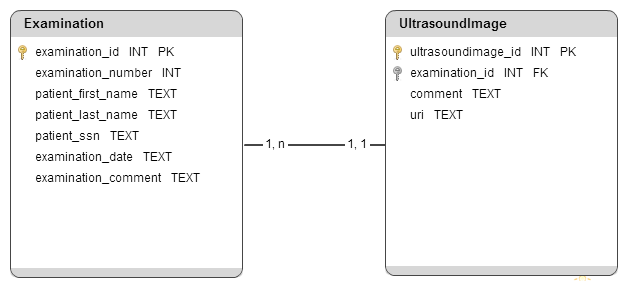
\includegraphics[scale=0.9]{img/database_design.png}}
\caption{Database design}
\label{fig:database_design}
\end{figure}

\noindent
Everything related to access to the database is handled by a class named \emph{DatabaseHelper.java}. The relationship between the database helper class and the data model classes is shown in Figure 18. DatabaseHelper has methods for adding, deleting, updating and retrieving \emph{Examinations} to/from the database. A point worth noting is that the data classes Examination and UltrasoundImage both implements \emph{Parcelable}. Parcelable allows for object instances to be written to and restored from a \emph{Parcel} \cite{parcelable}. This makes it possible to pass object instances from one activity to another via Intents without having to depend on temporary storage in the database. 

\begin{sidewaysfigure}
    \centering
    \label{fig:classdiagram_db_data}
        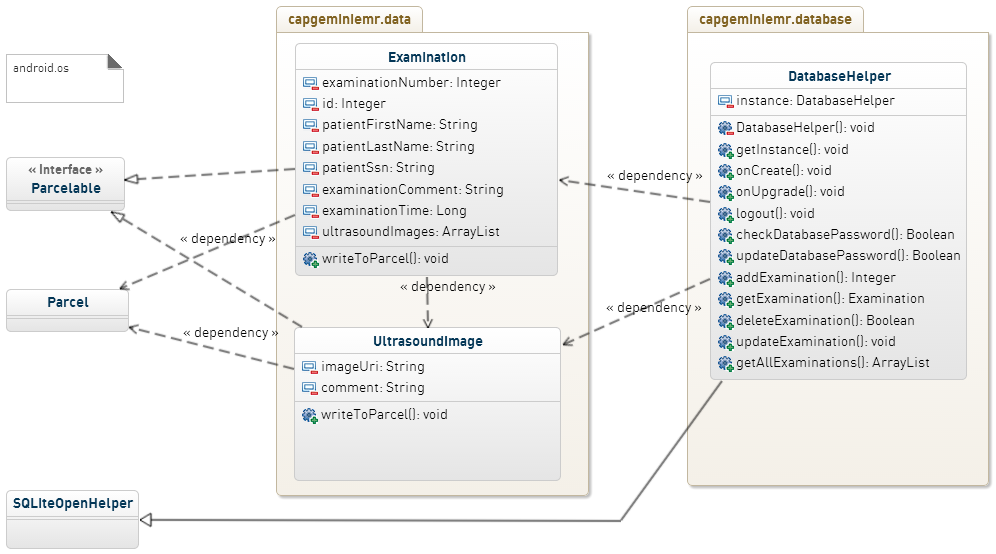
\includegraphics[scale=0.75]{img/classdiagram1.png}
        \caption{Class diagram: database and data}
\end{sidewaysfigure}


\newpage
\noindent
The DatabaseHelper class is used by multiple activities. In order to keep only one instance of this class that may be used throughout the application, we have implemented a \emph{singleton pattern}. Listing \ref{lst:database} shows the implementation of the singleton in \emph{DatabaseHelper.java}.

\begin{lstlisting}[caption={Singleton implementation}, label={lst:database}]
// DatabaseHelper.java
private static DatabaseHelper instance = null;

private DatabaseHelper(Context con, ArrayList<String> databaseInfo) {

        super(con, databaseInfo.get(0), null, DATABASE_VERSION);
        this.password = databaseInfo.get(1);
}

public static synchronized DatabaseHelper getInstance(
  Context con, ArrayList<String> databaseInfo) {

    if(instance == null) {
        SQLiteDatabase.loadLibs(con);
        instance = new DatabaseHelper(con, databaseInfo);
    }
    return instance;
}
\end{lstlisting}

\noindent
As described in section \ref{singletonArc}, the idea behind a singleton is that instead of letting other classes directly access the constructor and create new instances of the class, everything goes through a public method called \emph{getInstance(...)}. The constructor is therefore made private. The singleton class stores an instance of itself in a private field (appropriately named \emph{instance}). Every time some other class needs a \emph{DatabaseHelper}, they simply call the static method \emph{getInstance(...)} of DatabaseHelper instead of calling the constructor. This method will create a new instance of DatabaseHelper if the private field \emph{instance} is null and then return it. If not, it will return the existing instance instead of creating a new.

The reasoning behind using a singleton for the database helper is for performance reasons and the fact that no more than exactly one instance of the class will ever be needed. Performance is increased because the static method \emph{loadLibs(context)} of the SQLite database is an ''expensive'' operation when using SQLCipher and should therefore not be called more than needed.

\paragraph{Encryption}
The system uses two different encryption methods. To encrypt the database, the open source extension to SQLite called SQLCipher is used. To encrypt the password used to authenticate users, the cryptology package in Java is used. SQLCipher uses 256-bit AES (Advanced Encryption Standard) to encrypt all the database files. The Java cryptology implementation uses 128-bit AES encryption.

\subsubsection{Settings}

All necessary settings will be supplied to the application through an XML file containing all information needed for communication with external systems. This file is required to use the application. The first time the application is launched, the technical user will be prompted to enter the technical password to protect the technical part of the application. The layout of the XML file, as well as more in depth instructions for how to set up the application can be found in the technical manual (Appendix \ref{techmanual}). Once this password has been set, the user is required to supply an XML file containing all the communication settings for the application. The application will then parse the file, and save the settings to the \emph{SharedPreferences} of the application. The advantage of this is that non-sensitive data can be stored persistent, even when the application is closed or the device restarted.

A list of current settings can be found by choosing "View current settings" in the "Settings"-view. The technical password is required to access this page. To change the settings the user can choose to reconfigure the application. This will also require the technical password, and the user can once again supply an XML file with the new settings.

\subsubsection{Authentication and Session management}
\label{sessionimplement}
The application uses LDAP to authenticate users. All information needed to connect to the correct authentication server is supplied in the application settings. 
\noindent
LDAP is an application protocol used to query and modify items in directory services such as Active Directory. The application supports regular LDAP as well as LDAPS (LDAP over SSL). The process is described in Figure \ref{fig:login}.

\begin{figure}[H]
\centering
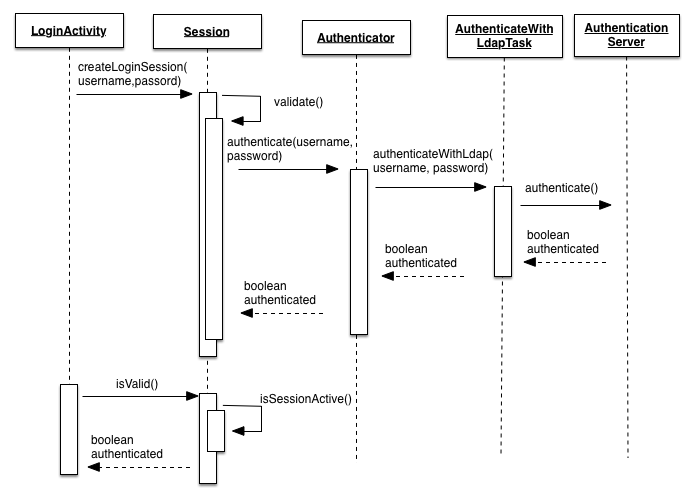
\includegraphics[scale=0.5]{img/sequence_auth.png}
\caption{Login}
\label{fig:login}
\end{figure}

\noindent
Even though LDAP was the only method implemented during this project, the application is designed to allow for the implementation of other authentication methods (such as Kerberos \cite{kerberos}) in the future.

To allow the user to easily switch between the application and the Vscan application, a session based system was designed. On a successful authentication a new session will be created. The session will store the username and a password hash to SharedPreferences and create a time stamp set to 10 minutes in the future. 

Every time the user navigates between activities in the application, a method in the session class will be called to check if the session is still valid, comparing the time stamp to the current time. This method will also check network connectivity, as a login session will not be valid if the user has lost connection. If the session is still valid, the time stamp will be updated. This way, the session will always be valid 10 minutes after the last interaction.

\subsubsection{AIDL and Services}

The AIDL interface is defined in a file with an \emph{.aidl} file extension. This file is supplied to both the application and the service. It is important that the file is in the exact same package on both ends. The service can then implement the Java interface generated by the AIDL file.

The application can use a method in the compiled AIDL file called \emph{Stub} to access the service interface. Before binding to a service, a new Intent is created, and its \emph{setClassName()} method is called with a reference to the package of the AIDL file and a reference to the actual service, both defined in the application settings. This intent is then supplied together with the actual Java interface to bind the service.

The final implementation of the AIDL interface consisted of two methods; one of them, identify patient method, would take in a SSN or similar identification numbers as a string, and return a list of information based on that number. The other function, upload images method, would take in three lists, one with patient information, one with images and one with comments to the examination and images. This method would return a Boolean variable reporting the success of the upload. Both methods also has a username field and a password field for communication with the hospital servers.
\begin{lstlisting}[caption={AIDL Interface}, label={lst:finalaidlinterface}]
// EMRRemoteInterface.aidl
package org.royrvik.emrservice;

interface EMRRemoteInterface {
    List<String> getPatientData(in String ssn, in String username, in String password);
    List<String> upload(in List<String> examinationData, in List<String> imagePaths, in List<String> notes, in String username, in String password);
}
\end{lstlisting}
\smallskip
The identify patient method was designed to hold the patient's SSN, while the return message would contain an array with the patient's first name and last name. The messages could however be easily modified, should the customer wish for additional data.

The upload images method is more complex, and contains three arrays; examination data, images and notes. Examination data contains all data from the examination, as well as the patient information, all in a well defined format (see Appendix \ref{devmanual}).
Images contains the path to the images, and notes contains the notes to each image.
\noindent
The response messages for both tasks is structured as an array. In addition to response data (i.e first name), the message contains a boolean \emph{didWork} together with an error message. Figure \ref{fig:service} describes the process for acquiring patient data, as well as uploading an examination for any service created for the application.   

\begin{figure}[H]
\centering
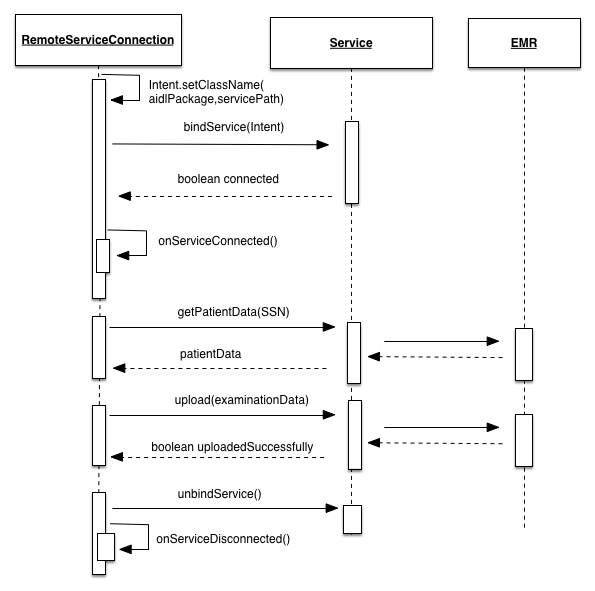
\includegraphics[scale=0.5]{img/sequence_service.png}
\caption{Application/Service communication}
\label{fig:service}
\end{figure}


\subsubsection{Offline Mode}
The offline mode functionality was implemented half way through the development process. This would strip all sensitive data from the application, while still enabling the user to edit the fields and view the images.
\noindent
At the end of the development process the database security was changed to use user credentials to encrypt the data instead of a static key. This caused the offline mode feature to lose database access when the user was unable to log in. The stripping functionality remained in the application, but the offline mode functionality itself was never implemented with the new database. 
\noindent
The group felt that a secure database was more important than a working offline mode, and prioritized more important parts of the application.

\subsubsection{Security}
As one of the projects quality attributes was security, the group spent a good amount of time figuring out how to secure the data storage. The techniques and tactics we used can be found in section \ref{architecturesecurity}. In the following section we will discuss how these tactics were implemented.

\paragraph*{Storage}
One of the biggest security issues of the project, was to store patient data safely on the device. As described in the architecture chapter, the choice fell on encrypting the database. The library used to encrypt the database file ensures that the file is encrypted at all times, which entails that the database remains secure even if the application should crash. Although implementing the encryption functionality was rather straight forward, figuring out how to handle the encryption key was a bigger struggle. It would of course defeat the purpose to have the encryption key in a code variable, and storing it elsewhere on the device was found to be unsafe. 

Storing it as a hash in Android's SharedPreferences was considered, since an application's SharedPreferences is restricted only to the application itself through UNIX permissions. This was quickly dismissed since research show that a rooted device, and its applications, would easily have its SharedPreferences compromised if an attacker wanted said information. Even if the encryption key was to be hashed, this would most likely only slow down the attacker. 

\noindent
Although the obvious and ideal solution to this problem is to have the encryption key as user input, but having users input a shared decryption key in addition to their own credentials was dismissed as unintuitive, impractical and unsafe. This would in addition put a lot of extra constrains on the user, which we - as stated in the USA5 quality attribute - wanted to avoid. 

The solution to this problem was to give each user their own database, where each database used the individual users password as encryption key. To know which database belonged to which user, it was decided that the name of each database file was the username of the user ("username".db). This also added a new feature to the application, as it is an industry practice to restrict the level of access medical personnel has after the “Not more than needed”  principle. Although this solution solved the main problem of safe storage, it also brought with it issues in regards to password policy. The application had to be able to handle a user password change, which happens frequently; once every third month at the hospitals the group had been talking to.

The application was now designed to have an encrypted database file for each user. If a new user was to log in, the application would detect this because no database with the name of the users username existed. In the same way the application would be able to determine if a user had changed his password, because he would be able to authenticate with the hospital servers (currently through LDAP), but not be able to decrypt the database. Functionality was therefore implemented to prompt for the users previous password to change the encryption key.

The implementation is not an optimal one, as it requires the user to remember both old and new password, but it was still chosen as the best solution by the group. A good argument for this solution, is that the workflow is structured so that an examination is to be uploaded within a reasonable time after it has taken place. If a password is still changed before the user has had time to upload the examination, it should still be fresh enough in his or her memory to not be a problem. If the user cannot remember his old password, the database can be deleted, so that a new database (with the new password) can be created. 


\subsubsection{Other Safety Measures}
Despite the safety measures described above in the security section, there were some worries related to the settings functionality. Given that an attacker somehow was able to steal a device, and put it back afterwards, the attacker could either switch the current service with a malicious service, and change the configuration so that the application sent sensitive data to that service. It was also a worry that the settings could be tempered with to such a degree, that data credentials could be sent to a malicious server. 
To counter this, it was determined that the technical user would set a password on the settings view so that no other then technician would be able to reconfigure the application. The settings file was changed to specify the name of the service, and an the settings view was changed so that any editing of the application settings would cause the entire database to be wiped.
According to the SEC2 requirement, no non-encrypted data should \emph{escape} the application, and be saved to disk. To fulfill this we have disabled the possibility to take screenshots while inside the application. Listing \ref{lst:disablescreenshot} shows how this was implemented.
\newpage
\begin{lstlisting}[caption={Screenshot disabling}, label={lst:disablescreenshot}]
getWindow().setFlags(WindowManager.LayoutParams.FLAG_SECURE, WindowManager.LayoutParams.FLAG_SECURE);
\end{lstlisting}



\subsection{User Manuals}

The group decided to divide the users into three user groups; 
\begin{itemize}
    \item Service developers 
    \item Technical staff
    \item Regular users 
\end{itemize}
This was done because a doctor (considered a regular user) should not need to know how the application works or the address and protocols for every connected server. Neither should technical staff at the hospital be required to know programming well enough to develop the service themselves.
The service development guide can be found in Appendix \ref{devmanual}. Technical manual is located in Appendix \ref{techmanual}, and user manual can be found in Appendix \ref{usermanual}.

\newpage
\subsection{Sprint summaries}
In the this section we will give a brief overview of our development process. Each week was documented by a weekly report. An example can be found in Appendix \ref{weekly_rep}.

\subsubsection{Sprint 1}
The group spent most of its time getting familiar with the task it was assigned, and furthermore how to approach the task in terms of work methodology. A draft of the projects requirements was developed, and the process of establishing a network of contacts from the industry was initiated. 
    
\subsubsection{Sprint 2}
In the beginning of this sprint, the initial requirements were in place. An architectural draft of the application was completed, and mockups of the GUI was finalized, tested and implemented. In regards to research, the group experienced a steep learning curve on the amount of systems used at hospitals. PACS, DICOM and how to communicate with hospital servers was the main focus as the group acquired contact in both OUS, DIPS and The Norwegian Directorate of Health. 


\subsubsection{Sprint 3}
The main focus of this sprint was research and implementing offline-mode functionality. The group also spent time to figure out how to actually communicate with different hospital information systems, and which protocols that needed to be used. During this process, a lot of emails were exchanged with contacts we had established with the industry.

During this sprint's research, the group was made aware that not all medical personnel can use PACS for storing images. Since this was the system the customer initially had suggested that the images should be uploaded to, further research into other systems was needed.

\subsubsection{Sprint 4}
\label{sprint4}
At this stage, the group realized that rules and regulations as of today prevented us from uploading images from mobile devices to a hospital information system (see \ref{multimediaInHospitals}). Nevertheless, together with the customer we decided to ignore this, and focus our work on figuring out how to upload data to the PAS/EMR, just as a proof of concept. Alongside with this, the customer also wanted us to explore future solutions in greater depth.

In parallel with the research that was done, a lot of the applications core functionality was implemented. This included the SQLite database, settings, authentication, sessions and QR code scanning.   


\subsubsection{Sprint 5}
In sprint 5 the final architecture of the service was designed. Building on the new architecture, the group worked on creating a service that would communicate with a DIPS BizTalk server, given to us by Sykehuspartner. This was intended to be a dummy DIPS service, illustrating the functionality of the new service implementation.

BizTalk technology required communication to happen through C\#. The group had to do research both on the Windows Communication Framework/.NET, as well as how to make C\# code run on Android.

Because of technical issues with the DIPS server, a simple backup service using MySQL and SFTP was developed instead. During this sprint a lot of security features were also added, including database encryption.    


\subsubsection{Sprint 6}
This sprint was used to complete the development process, as well as producing a first draft of the final report. 

During the sprint, the backup service was completed and the communication between the application and the service was standardized and documented. The user interface went through a complete overhaul, giving it a clean look and feel. A new "Full Screen Image"- view was also implemented, making it easier to view and comment on images. In addition to this, a lot of time went into fixing known errors and bugs.